\documentclass{sig-alternate}

% UTF8 support
\usepackage[utf8x]{inputenc}

\usepackage{subfig}
\usepackage{hyperref}
\usepackage{graphicx}
\graphicspath{{figures/}}

\usepackage{booktabs}

\newcommand{\eg}{{\textit{e.g.~}}}
\newcommand{\etal}{{\textit{et al.~}}}
\newcommand{\ie}{{\textit{i.e.~}}}

\usepackage[draft,footnote,nomargin]{fixme}

%
% --- Author Metadata here ---
\conferenceinfo{10th ACM/IEEE International Conference on Human-Robot Interaction}{2015 Portland, USA}
%\CopyrightYear{2007} % Allows default copyright year (20XX) to be over-ridden - IF NEED BE.
%\crdata{0-12345-67-8/90/01}  % Allows default copyright data (0-89791-88-6/97/05) to be over-ridden - IF NEED BE.
% --- End of Author Metadata ---

\title{\LARGE \bf
    Eye-Tracking: a New Look at Human-Robot Interaction Assessment
}

%%% HRI 2015 -> double-blind review process
%
%\numberofauthors{1} 
%\author{
%\alignauthor
%Kshitij Sharma, S\'{e}verin Lemaignan, Pierre Dillenbourg\\
%       \affaddr{Computer-Human Interaction in Learning and Instruction Lab (CHILI)}\\
%       \affaddr{Ecole Polytechnique F\'{e}d\'{e}rale de Lausanne (EPFL)}\\
%       \affaddr{CH-1015 Lausanne}\\
%       \affaddr{Switzerland}\\
%       \email{firstname.lastname@epfl.ch}
%}
%
%\additionalauthors{Additional authors: 
%Francesco Mondada, LSRO, EPFL, francesco.mondada@epfl.ch 
%}
%

\begin{document}
\maketitle
\begin{abstract}


Eye-tracking has been previously shown to be an effective proxy to understand
complex socio-cognitive interactions. Yet its application to human-robot
interactions (HRI) remains limited. This article presents the state of the
art in eye-tracking methods for interaction assessment, and explores how those
are applicable to HRI.

Techniques based on mobile eye-tracking as well as the main analysis approaches
for eye-tracking data are first exhaustively presented, with an emphasis on
those we believe relevant to robotics. We then report on a study involving the
educational robot Thymio II~\cite{riedo2012two} with 52 participants: the
students have to explain a pre-programmed behaviour of the robot with or without
the help of visual cues. The study setup and analysis illustrate how to apply
eye-tracking techniques to actual human-robot interaction situations.

\end{abstract}
%%%%%%%%%%%%%%%%%%%%%%%%%%%%%%%%%%%%%%%%%%%%%%%%%%%%%%%%%%%%%%%%%%%%%%%%%%%%%%%%%%%%
%%%%%%%%%%%%%%%%%%%%%%%%%%%%%%%%%%%%%%%%%%%%%%%%%%%%%%%%%%%%%%%%%%%%%%%%%%%%%%%%%%%%
\section{Introduction}

Eye tracking provides unprecedented access to the users' attention and
engagement during interactive scenarios. Previous research\fixme{refs} has shown
that gaze data can be used as a proxy to understand the underlying
socio-cognitive aspects in not only human-computer interaction but in
human-human interaction as well. In the present decade, off the shelf
eye-trackers have become readily available to the researchers to assess
the users' attention and engagement.

On the other hand, educational robots can be of great use in making young school
kids interested in technological developments~\cite{cooper1999robots,
wyffels2010building}. It is important to know about the key socio-cognitive
features of this subset of human-robot interaction because these features let
the researchers design better interactive scenarios in the future. These
features include the conceptual mapping of the sensor data visualisation and the
robot's function and the generalising the concepts to solve a given problem in a
contextual learning environment.

Thymio II~\cite{riedo2012two} can provide salient effects onto our visual
attention through the LEDs. We can use this feature to guide the users'
attention in a way that the effectiveness of the interaction is maximised. In
the case of interaction with the educational robots the effect of the
interaction is to make the users understand the technical aspects of the robot
and to make the users be able to transfer it to different domains.

We propose to use the mobile eye trackers to be able to have our participants
freely move on the experiment site. Using mobile eye tracker poses a technical
challenge to automatically locate where the participants are looking. This is
not a trivial task as the visual stimulus for participants is changing with
every bit of motion of their head. This is the reason we used fiducial-markers
on the maze we used in the experiment so that we can reconstruct the whole maze
even if only a part of it is the visual field of the participant.


\paragraph{Biometric Measurements of Interaction}

\fixme{organize/rewrite this paragraph}

\fixme{Mention skin conductance as well}

Evaluation of HRI is mostly done through qualitative questionnaires and
qualitative data (interaction videos, interviews for example). The physiological
measurements such as eye tracking being precise, pertinent and portable at the
same time provides an added value to the researcher.  However, this needs to be
complemented with the qualitative data as well.


Eye-tracking data is of high temporal precision as
compared to some of the physiological data sources such as fMRI or other
biometric devices used to measure the palpitation and the body temperature. The
eye tracking devices are portable enough as opposed to the bulky apparatus used
in fMRI~\cite{rosenthal2013neural}.  Eye tracking data provides more direct
access to the users' attention than other portable and physiological data
sources such as EEG; this makes eye-tracking data a pertinent source to measure
attention.

The prime advantage of using mobile eye-tracking is that the users' interaction
with the robot can still be ecologically valid. On the other hand, using fMRI
for evaluating HRI reduces the interaction to a video of the robot only
~\cite{rosenthal2013neural}.

Another advantage of using mobile eye-tracking to assess HRI situations, is that
the data provides direct and noise free access to the users' attention. While in
other physiological measures for attention, such as EEG, the data has a lot of
noise and the relation to the attention is very task-specific.


%Our working hypothesis is that with careful mapping between the LED
%visualisations and the behaviour of the robot we can induce the understanding of
%the functionality of the robot very easily. We propose to use the gaze data to
%verify this hypothesis. With eye-tracking data we can judge whether the mapping
%between the behaviour and visual actuators is useful or not for the participants'
%understanding.  Moreover, we hypothesise that the good performers will be able
%to anticipate the robot's motion. Eye-tracking data can also be useful to verify
%the anticipation hypothesis.
%
%The experiment consists in two phases. The first phase is the observation phase
%during which the participants watch the robot move and detect an obstacle in a
%``playground''. The second phase requires the participants to interact with the
%robot by placing an obstacle in its path to make it detect the obstacle before
%reaching a certain target.  After each phase the participant explain the
%behaviour of the robot. The sensor data was visualised through LEDs with three
%visualisation conditions: {\sf TRUE} visualisation, {\sf RANDOM} visualisation and {\sf NONE}
%visualisation. Through this experiment we investigate the following research
%questions:
%
%\begin{enumerate}
%    \item Are there different gaze patterns for different levels of performance
%during the interaction? Moreover, can we see any anticipation patterns
%for the good performers?
%
%    \item How does displaying the sensor information on the robot' body as a
%visual cue affects the gaze and performance of the participants?
%\end{enumerate}
%
%The rest of the paper is organised as follows. The second section gives
%a brief review of the eye-tracking research done to quantify the
%expertise and performance. The third section presents the specificities
%of the study. The fourth section lists the main results. The fifth
%section discusses the results. Finally, the sixth section concludes the
%paper.

%%%%%%%%%%%%%%%%%%%%%%%%%%%%%%%%%%%%%%%%%%%%%%%%%%%%%%%%%%%%%%%%%%%%%%%%%%%%%%%%%%%%
%%%%%%%%%%%%%%%%%%%%%%%%%%%%%%%%%%%%%%%%%%%%%%%%%%%%%%%%%%%%%%%%%%%%%%%%%%%%%%%%%%%%
\section{Eye Tracking as a Tool for Assessing Social Interaction}

\subsection{Gaze patterns and Expertise/Task based performance}

Several scholars related gaze patterns with level of expertise.
\cite{hasse2012measure} in an air traffic-monitoring task found out that the
experts looked less at the scenario-specific information than novices.
\cite{eivazi2012gaze, law2004eye, tien2010measuring} studied the effect of
expertise on the gaze patterns in different surgical tasks and concluded that
experts look less at the instruments than the novices, instead they focus more
on the task specific areas. \cite{reingold2001visual} showed that expert chess
players pay more attention to the relative positions of the pieces, rather than
the individual pieces, than novice chess players. \cite{blignaut2008visual} also
studied the difference between experts and novice chess players in a checkmate
avoidance task and concluded that the experts have more gaze falling on the
important squares than the novices. In a program-debugging task,
\cite{sharif2012eye} showed that the expert programmers scan through all the
lines in the program faster than the novices. In a Tetris game,
\cite{jermann2010using} showed that experts pay more attention to the stack of
Tetronimoes while novices allocate more attention to the new pieces falling from
the top.

\subsection{Gaze patterns and Collaborative performance}

Previous work also show a clear relation between gaze patterns and
task-based performance in collaborative settings. As a measure of joint attention in collaborative settings  \cite{richardson2007art} proposed gaze recurrence between the collaborators and showed it to be correlated with the collaboration quality of the pair. In a pair-programming task, \cite{jermann2012effects} showed that the good performing pairs have more synchronised gaze on different parts of a program than the bad performing pairs. In a similar task, \cite{sharma2012gaze} showed that the good performing pairs pay more attention to the data-flow of the program than the poor performing pairs. Moreover, \cite{sharma2013understanding} showed that while describing the functionality of a program the well performing teams had more gaze on the variable modification parts in the program while poor performing teams have equal distribution of gaze on different parts of the program during similar phase of the task.  Thus we see that previous research provides insights about the relationship between the gaze patterns and the behavioural and task-based performance indicators in diverse scenarios.



%%%%%%%%%%%%%%%%%%%%%%%%%%%%%%%%%%%%%%%%%%%%%%%%%%%%%%%%%%%%%%%%%%%%%%%%%%%%%%%%%%%%
%%%%%%%%%%%%%%%%%%%%%%%%%%%%%%%%%%%%%%%%%%%%%%%%%%%%%%%%%%%%%%%%%%%%%%%%%%%%%%%%%%%%


\section{State of Eye Tracking in Human-Robot Interaction}

The usage of eye-tracking methods in HRI is very sparse. It must be noted that to our best knowledge only very few attempts to use eye-tracking as an interaction modality or as an interaction assessment technique in HRI.

\subsection{Eye Tracking as an Interaction Modality}

To guide the motion of a robot \cite{bhuiyan2004tracking} used real time  gaze data of a human user. The users were able to provide the visual and geometrical motion information to the robot by moving their eyes in different parts of the human-robot interface.

\subsection{Eye Tracking as a tool to Assess Interaction Algorithms}

To evaluate the effectiveness of the motion planning algorithm for a robot \cite{dehais2011physiological} used eye-tracking techniques. In an object hand-over task between a robot and a human, the authors compared various motion planning algorithms based on the gaze of the human.

\subsection{Eye Tracking as a tool to Assess Joint Attention}

 In an eye-tracking study, in the context of human robot interaction, \cite{staudte2009visual} found
that when the robot provides a matching visual and verbal reference to an object
the participants were more likely to look at the correct objects. This result
was consistent irrespectively of the ambiguity of the situation. The video based interaction modality was used by the authors. This constraints the  interaction of the human-robot dyad to just a video. However, the stimulus (video) for eye-tracking provides strong contrast and a good control for experimental conditions.






%%%%%%%%%%%%%%%%%%%%%%%%%%%%%%%%%%%%%%%%%%%%%%%%%%%%%%%%%%%%%%%%%%%%%%%%%%%%%%%%%%%%
%%%%%%%%%%%%%%%%%%%%%%%%%%%%%%%%%%%%%%%%%%%%%%%%%%%%%%%%%%%%%%%%%%%%%%%%%%%%%%%%%%%%

\section{Method description}

%%%%%%%%%%%%%%%%%%%%%%%%%%%%%%%%%%%%%%%%%%%%%%%%%%%%%%%%%%%%%%%%%%%%%%%%%%%%%%%%%%%%
%%%%%%%%%%%%%%%%%%%%%%%%%%%%%%%%%%%%%%%%%%%%%%%%%%%%%%%%%%%%%%%%%%%%%%%%%%%%%%%%%%%%
\subsection{Eye-tracking}


\subsubsection{Apparatus}
\begin{enumerate}
\item Stationary
\item Mobile 
\item Dual eye-tracking

\end {enumerate}


\subsubsection{Mobile Eye-tracking setup}

\begin{enumerate}
\item Calibration
\item Recording Scene 
\item Recording Gaze

\end {enumerate}

\subsubsection{Use cases for mobile eye-tracking} 

\begin{enumerate}
\item Stationary target, stationary observer
\item Moving target, stationary observer
\item Stationary target, moving observer
\item Moving target, moving observer
\end{enumerate}


\subsection{Data and Analysis}

\begin{enumerate}
\item Fixations: The most common form of eye-tracking data aggregation are the fixations.
Fixations depict the periods in the user's observation when the user
attends a relatively small part of the visual stimulus for a relatively
longer period of time. The various fixation detection algorithms are
summarised in~\cite{duchowski2007eye}. 

\item Saccades and transitions
\item Smooth Pursuit
\item Areas of Interest
\item Heat-maps

\end {enumerate}


\subsection{Joint attention and social behaviour analysis}


\section{Method Application Example}

\subsection{Setup and Conditions}

Thymio II is a small robot designed for education for 6 to 16 year old
children~\cite{magnenat2012programming, riedo2012two}. Users can interact with
it via buttons and distance sensors. The robot can display its states via many
LEDs and its motion. We programmed it to show the value of the front IR-sensor
on its top. The display consists of 8 LEDs (Figure~\ref{thymio}).

In the experiment, there were 3 sensor data visualisation conditions.  For the
{\sf TRUE} visualisation condition, the number of illuminated LEDs, on the top of the
robot, is proportional to the intensity measured by the IR-sensor. When the
intensity of the reflected IR crosses a predefined threshold, the robot does a
90° turn to its right. For the two other conditions, the behaviour is the same,
simply the display changes. In the {\sf RANDOM} condition, the display shows as if the
robot was detecting the obstacle at random moments, while in the {\sf NONE}
visualization condition nothing is shown on top of the robot. The robot has a
fitting for a pencil that we used for the drawing of its trajectory.

\begin{figure}
    \centering
    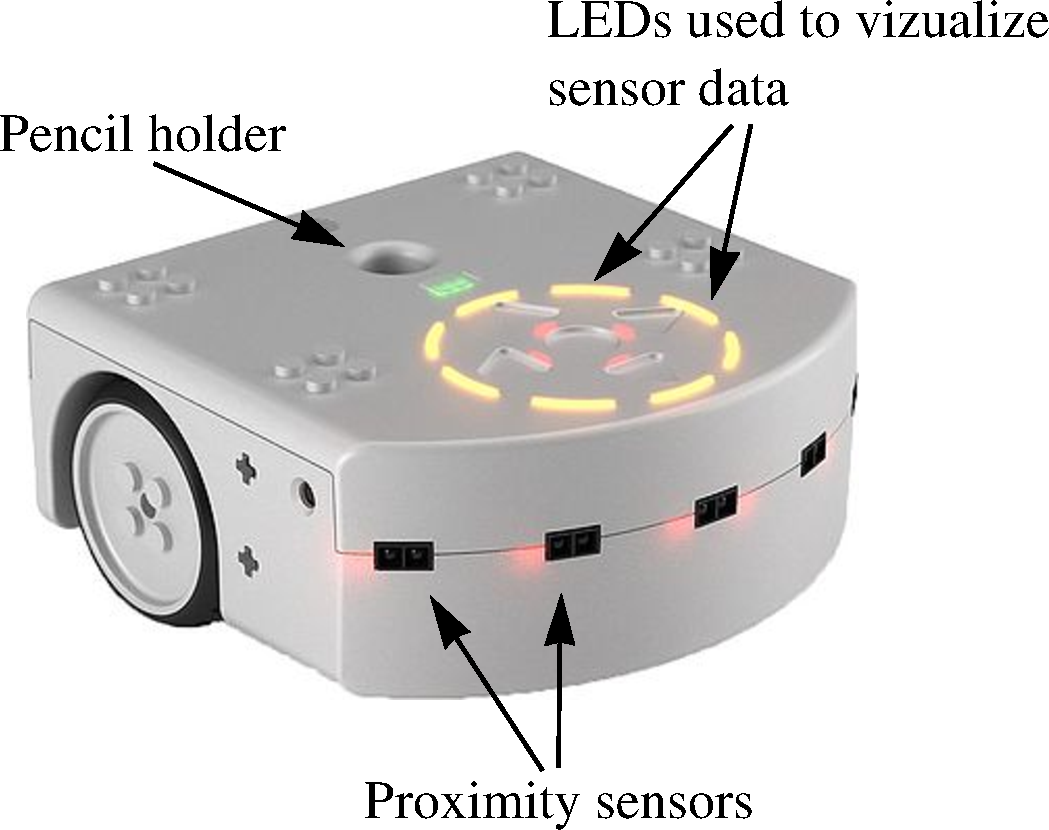
\includegraphics[width=0.9\linewidth]{thymio}
    \caption{\small \textbf{Thymio II}: the proximity sensors were used to
    detect the obstacle based on the reflectance of the material. The sensor
    data was shown as a proportion of the circle lit using the LEDs on top of the
    robot.}

    \label{thymio}
\end{figure}

The playground (Figure~\ref{playground}) is designed in order to allow the
participants to get a reference of the previous behaviour of the robot, as well
as to allow us to localise the position of the robot, the position of the
obstacles and the position of the gaze on the video recorded from the
eye-tracker. The localisation is made possible by the use of unique fiducial
markers on the playground. On the right hand side, the observation phase takes
place and there will be the reference for the black and white obstacles. On the
left hand side, the interaction takes place.

\begin{figure}
    \centering
    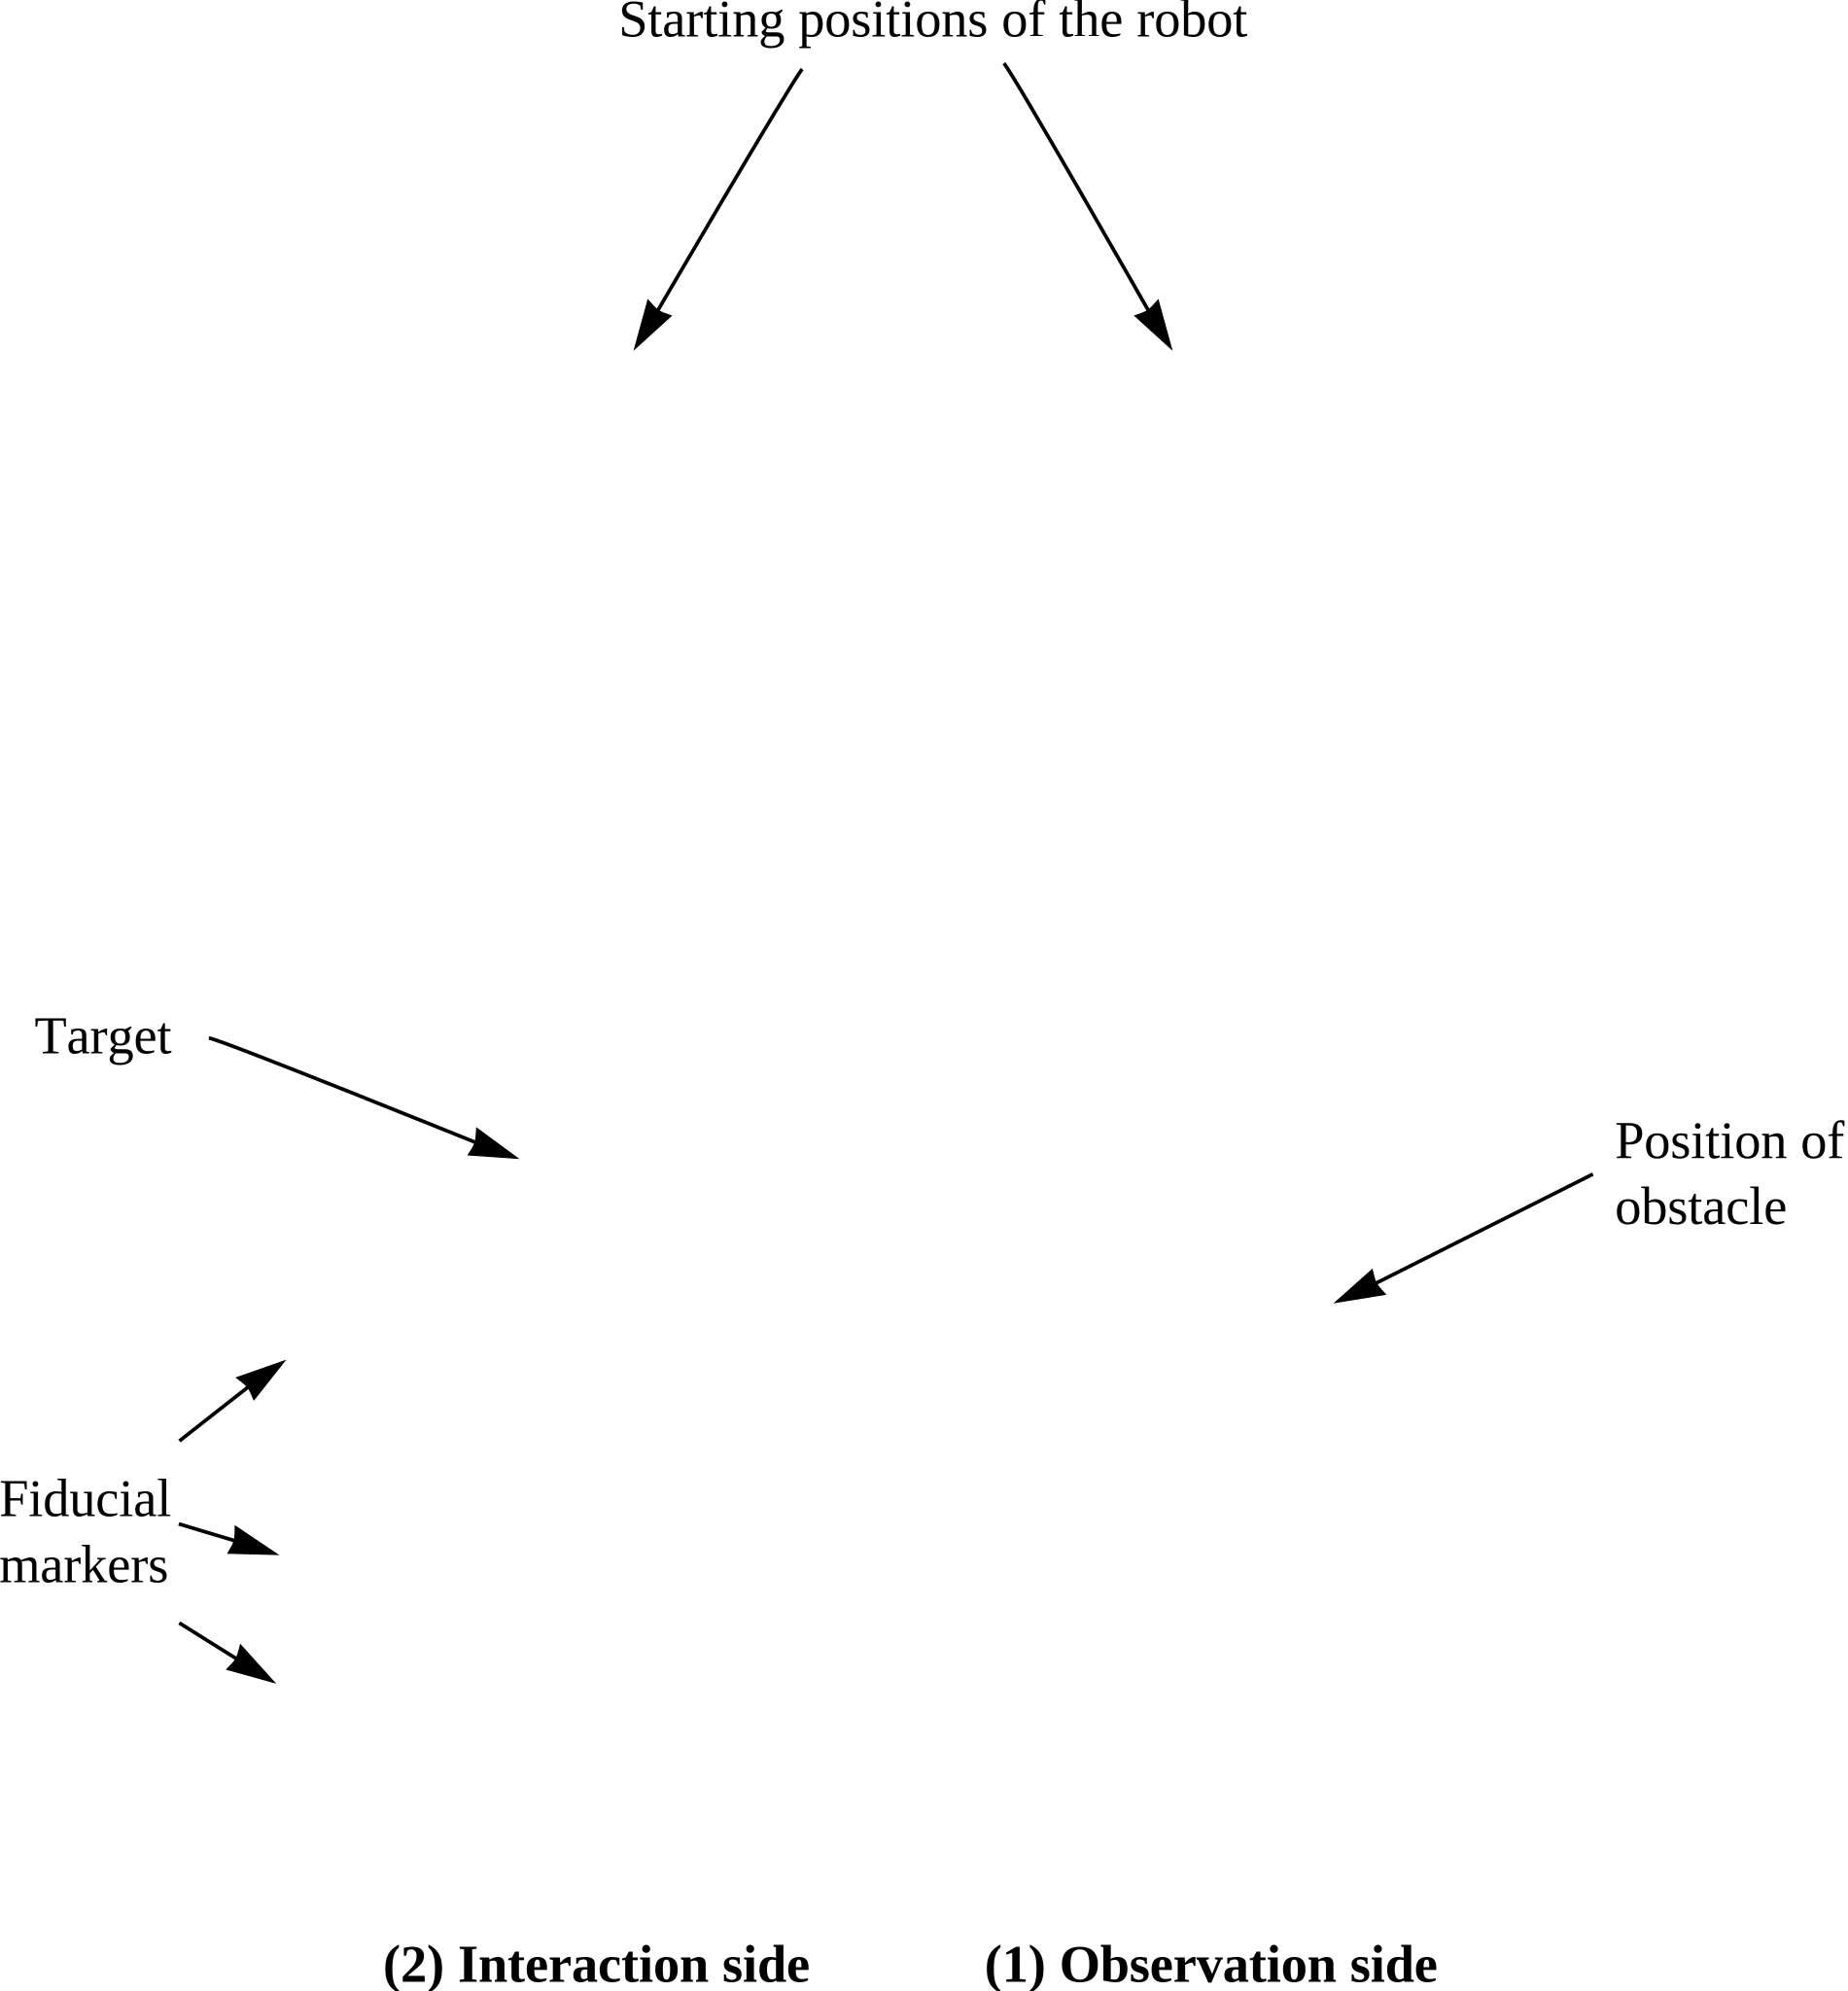
\includegraphics[width=0.9\linewidth]{maze}
    \caption{\small Basic playground for the experiment. The fiducial markers
    are used for automatic localisation of the gaze pointers on the observation
    video.}

    \label{playground}
\end{figure}

One important fact to be considered is that the localisation of the
robot, the obstacle or the gaze pointer on the observation field for the
participant is not a trivial task. The fact that the participants are
free to move, poses a challenge to the eye-tracking analysis. The
movement of the participant causes change in the observation field of
the participant almost every frame of the eye-tracking video. To cope up
with the changing observation field we decided to put an array of
fiducial markers on the playground. Using the fiducial markers enabled
us to recreate the whole playground for every frame in the video
recorded from the eye-tracker's camera (Figure~\ref{expe}).

\subsection{Procedure}

Upon their arrival at the experiment site, the participants signed a
consent form and answered a small questionnaire about demographics and
participant's experience with educational robots (this we later consider
as expertise). The participants were placed in front of the playground
(Figure~\ref{expe}) and were equipped with the SMI eye-tracking glasses. The
actual experiment consisted in two phases: observation phase and
interaction phase.

\paragraph{Observation phase} The participant observes the Thymio II robot
approaching obstacles. The robot turns as soon as it detects the
obstacle. The participant watches the robot's behaviour for a black and a
white obstacle for 5 trials each. For the white, the robot turns
earlier; for the black obstacle the robot turns later. In the final
trial the robot is equipped with a pen to draw its trajectory for both
obstacles with different colours. After drawing, the participant is asked
the question: ``How does the robot work?''

\paragraph{Interaction phase} In the second phase, the participant is asked
to guide the robot to a goal, using a grey obstacle. The participant can put the
obstacle wherever he likes on the left hand side (Figure~\ref{playground}) of
the playground before the robot starts. We designed the grey obstacle to reflect
more infrared light (IR) than the black or the white obstacles therefore the
robot turns even earlier. This leads to a surprising effect. The participant has
only the robot's trajectories as a source of information. Each participant is
given 5 trials to put the obstacle in order to guide the robot to the goal. The
participant then has to answer the same question as in the observation phase,
response to which is considered as a final answer.

\begin{figure}
    \centering
    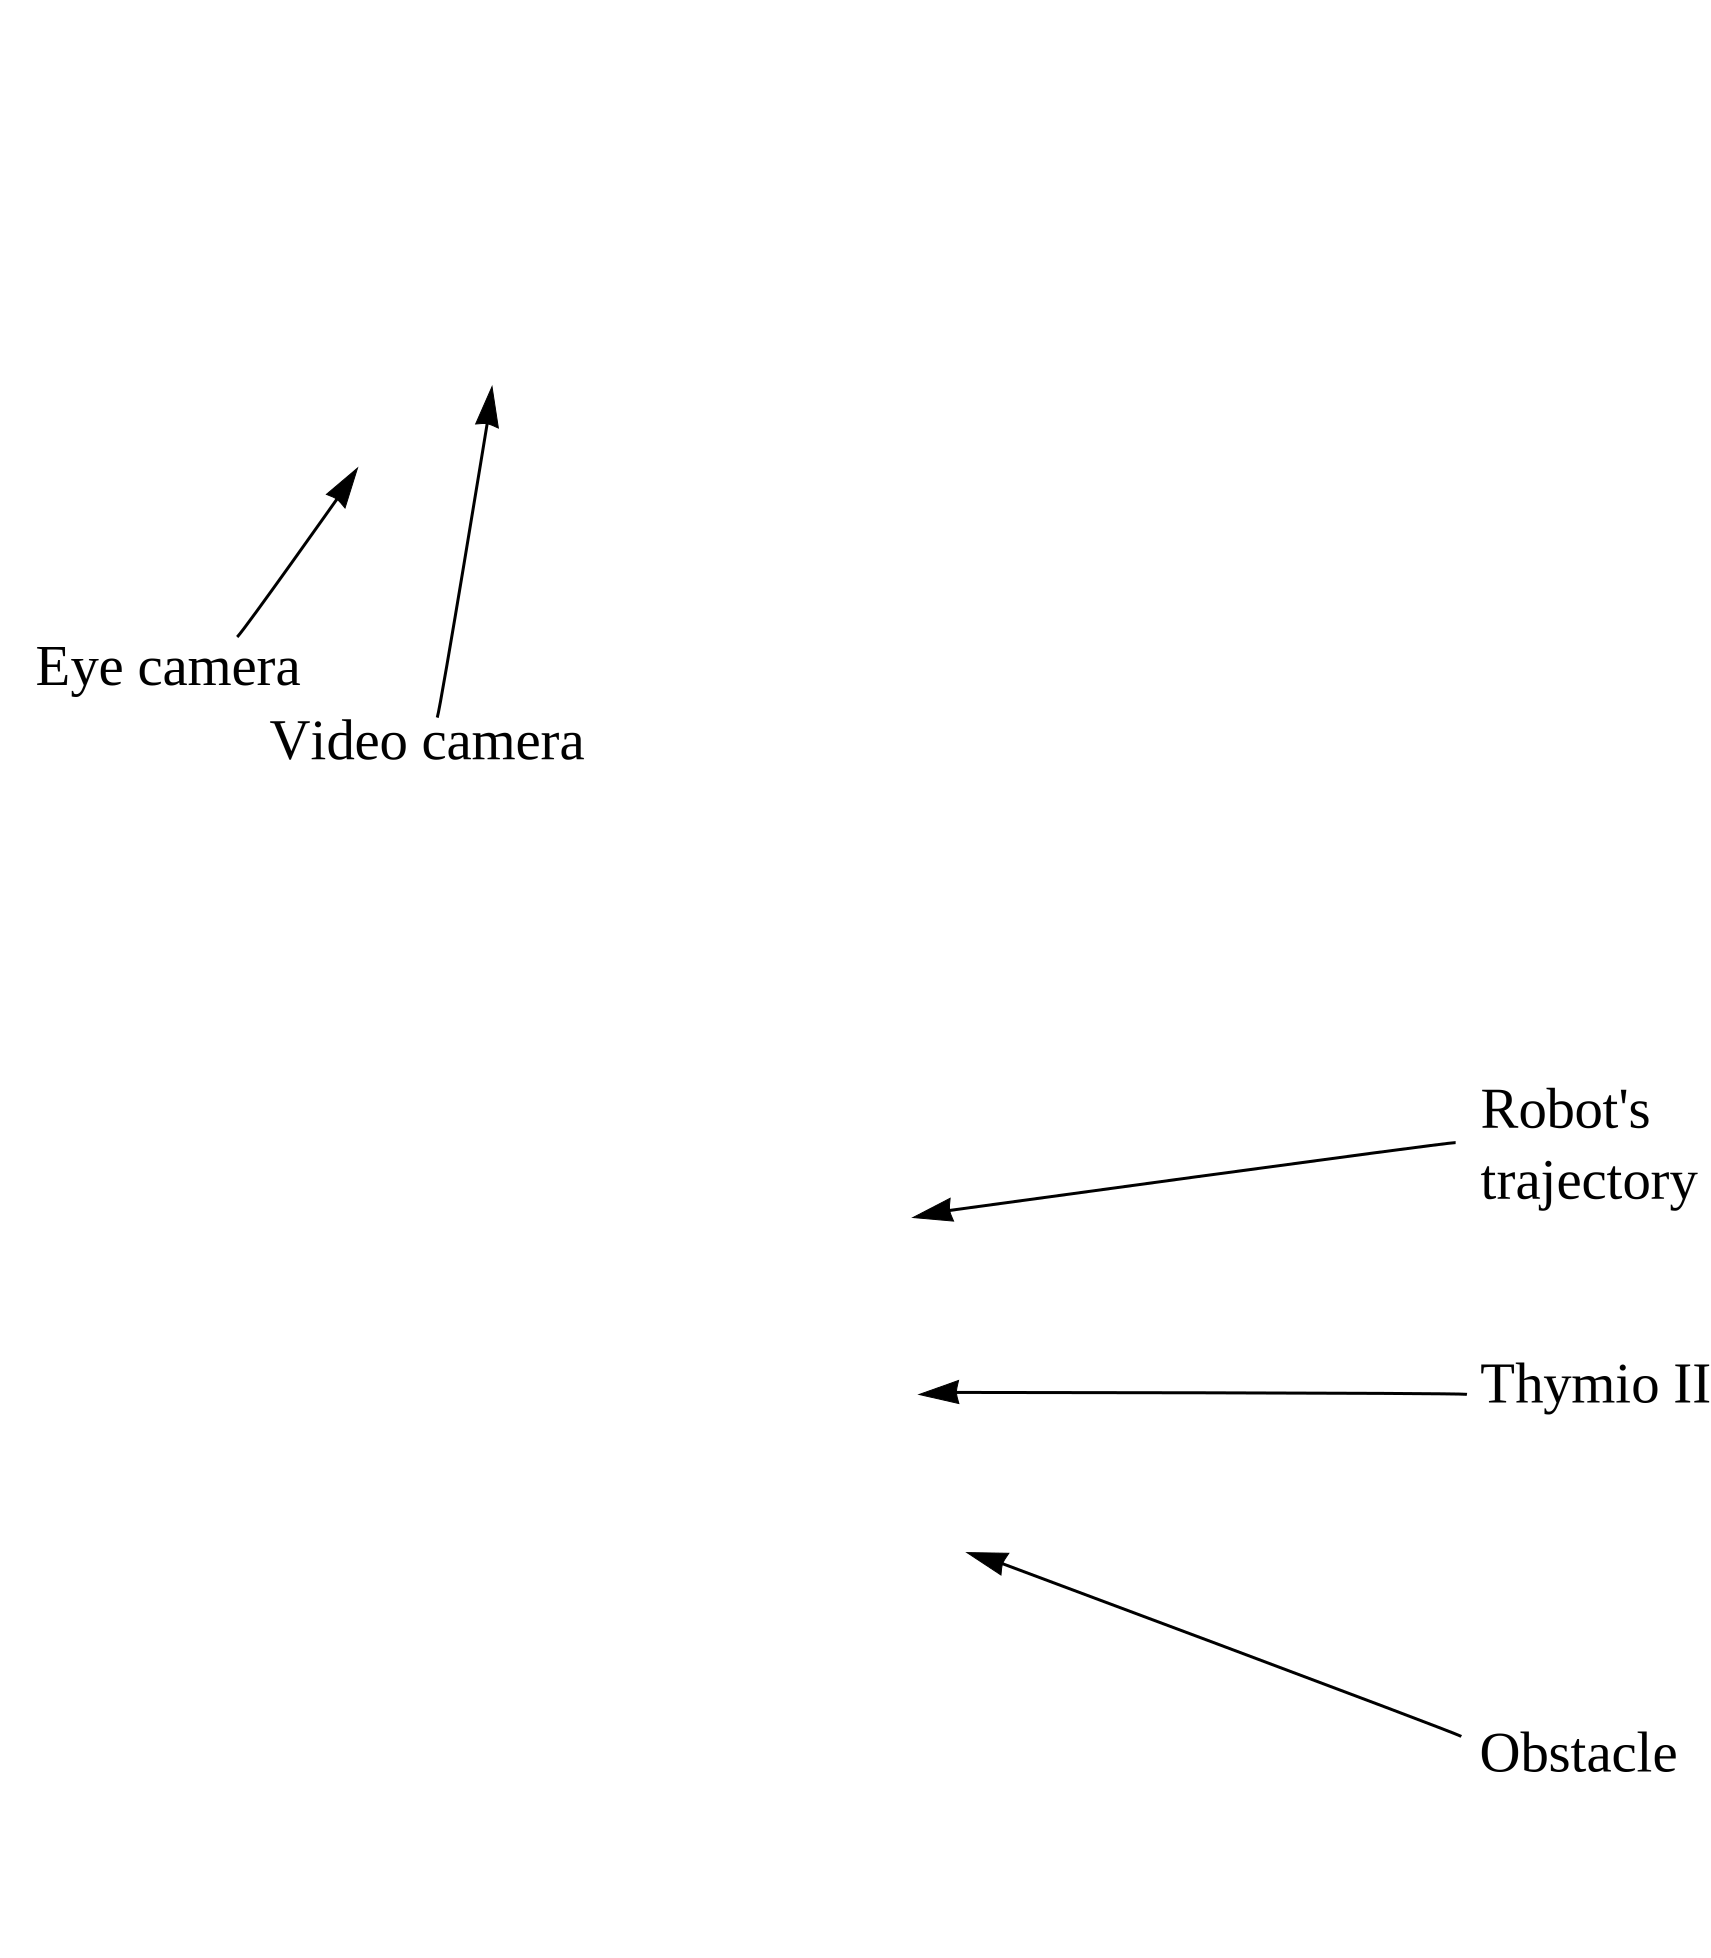
\includegraphics[width=0.9\linewidth]{setup}
    \caption{\small Experimental setup for observation phase. The observation
    video is recorded from the video camera in the front of the eye tracker (in
    the lop-left corner).}

    \label{expe}
\end{figure}

\subsection{Participants}

We recruited 52 participants for the experiment. All of them were
students from École Polytechnique Fédérale de Lausanne, Switzerland.
Most of them were in their first year undergraduate program (with two
exceptions). ~The age distribution was narrow, with a mean of 19.7 and a
standard deviation of 1.97. There were 13 female and 39 male
participants. In the three experimental conditions, {\sf NONE}, {\sf RANDOM} and
{\sf TRUE}, there were 18, 17 and 17 participants respectively.

\subsection{Eye-tracking measures}

Average fixation duration on the robot: We measured the amount of time a
participant looks at the robot and averaged this duration for the number
of fixations on the robot for the particular participant.

Average fixation on the reference side: The main area (right hand side
of figure 2) in the observation phase is treated as the reference side
in the interaction phase. The rationale behind keeping the lines drawn
by the robot in the observation phase is for the participants to be able
to refer to the prior behaviour of the robot in the interaction phase. We
measured the amount of time a participant looks at the reference side
and averaged this duration for the number of fixations on the reference
side for the particular participant.

\subsection{Performance measures}

%We had two measures of performance. First measure was a rating given to
%the responses that participants gave to the question about the
%functionality of the robot. Second measure was the distance from the
%target in the interaction phase.

%We transcribed the responses to perform a rating scheme on the level of
%abstraction and correctness. A low level of abstraction consists in
%describing the functionality of the robot in the terms of the electric
%or programming aspects of the robot, a high level represents describing
%the behaviour. For the levels of correctness, we categorised the
%responses into correct or incorrect response. In TABLE I. we present
%sample responses for the different categories.

%\begin{table}[ht!]
%    \centering
%    \footnotesize
%    \begin{tabular}{ccp{4.5cm}}
%        \toprule
%        Correct. & Abstract. & Sample answer \\
%        \midrule
%        \textit{incorrect} & \textit{low} & ``The robot turns at a given distance in respect to a colour, defined in the program.''\\ 
%        \midrule
%        \textit{incorrect} & \textit{high} & `Grey is the most dangerous, so the
%        robot turn really early.''\\ 
%        \midrule
%        \textit{correct} & \textit{low} & ``The grey obstacle reflects a lot,
%        the robot sends light. At a certain threshold the robot turns.'' \\ 
%        \midrule
%        \textit{correct} & \textit{high} & ``The grey obstacle is shinier, so
%        more reflective, and better detectable.''\\ 
%        \bottomrule
%    \end{tabular}
%    \caption{Sample answers for all classes}
%
%    \label{sample_answer}
%\end{table}

We measured the distances from the target were measured for all 5 trials. As
a matter of fact, as soon as the principle of the robot was deemed to be
understood by the participants, almost all the participants behaved the
same way. On the first try almost every participant failed and the robot
turned instantly. So the most significant distance measure was the
improvement between the first and second trial. It is referred to as
improvement in the following sections.

%Incorrect answers were further classified into 4 categories; we present
%each category accompanied by a sample response:
%
%\begin{itemize}
%    \item The participant did not respond or offer a possible explanation: ``I
%        really don't know how the robot works''.
%
%    \item The participant identified a wrong cause for the behaviour of the robot:
%        ``The robot notices the tags on the side''.
%
%    \item The participant held the code responsible for the cause of different
%        behaviour: ``The robot turns at a given distance in respect to a color,
%        defined in the program''.
%
%    \item The participant tried to explain by analogies or did not explain the
%        robots behaviour at an understandable level: ``Grey is the most
%        dangerous, so the robot turns really early''.
%
%\end{itemize}

%%%%%%%%%%%%%%%%%%%%%%%%%%%%%%%%%%%%%%%%%%%%%%%%%%%%%%%%%%%%%%%%%%%%%%%%%%%%%%%%%%%%

\subsection{Results}

We found no bias for age, gender, expertise, student status or condition
in respect to the correctness, abstraction and type of mistake made for
the final answer. Surprisingly there is no correlation between the
visualisation condition and the correctness or abstraction of the
answers given. We could not find any anticipation patterns in the
eye-tracking data. We found some other relation between the different
measures. We present the results in following subsections.

\subsubsection{Average fixation duration on the robot during observation phase
vs.~condition}

The average fixation duration on the robot during observation phase
(Figure~\ref{res1}) is significantly more in {\sf TRUE} and {\sf RANDOM} condition than in
the {\sf NONE} condition ($F[2,49]=3.68$, p = .03). This depicts that the
sensor data visualisation has an effect on the users' attention.

\begin{figure}[h!]
    \centering
    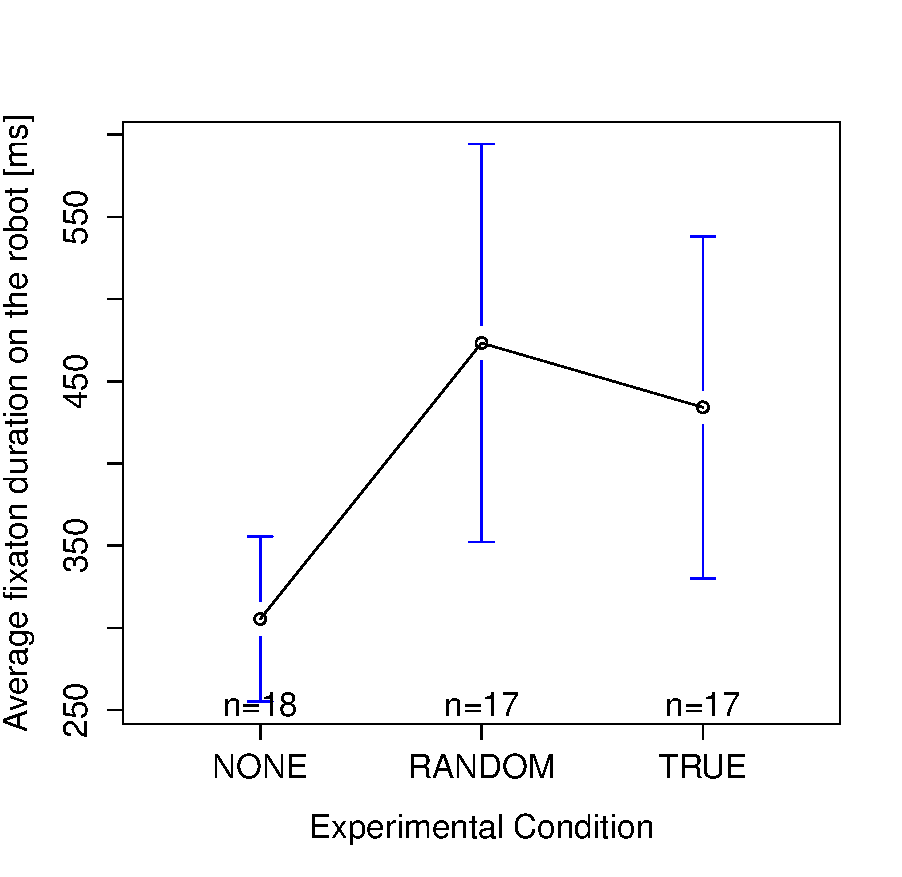
\includegraphics[width=0.8\linewidth]{meanPlotFixRobo}
    \caption{Average fixation duration on the robot ~during the observation phase
    vs.~Condition}
    \label{res1}
\end{figure}

\subsubsection{First improvement vs.~condition}

The first improvement is significantly more in {\sf NONE} and {\sf RANDOM}
conditions (Figure~\ref{res2}) than in the {\sf TRUE} condition ($F[2,49]=3.75$, p =
0.03).

\begin{figure}[h!]
    \centering
    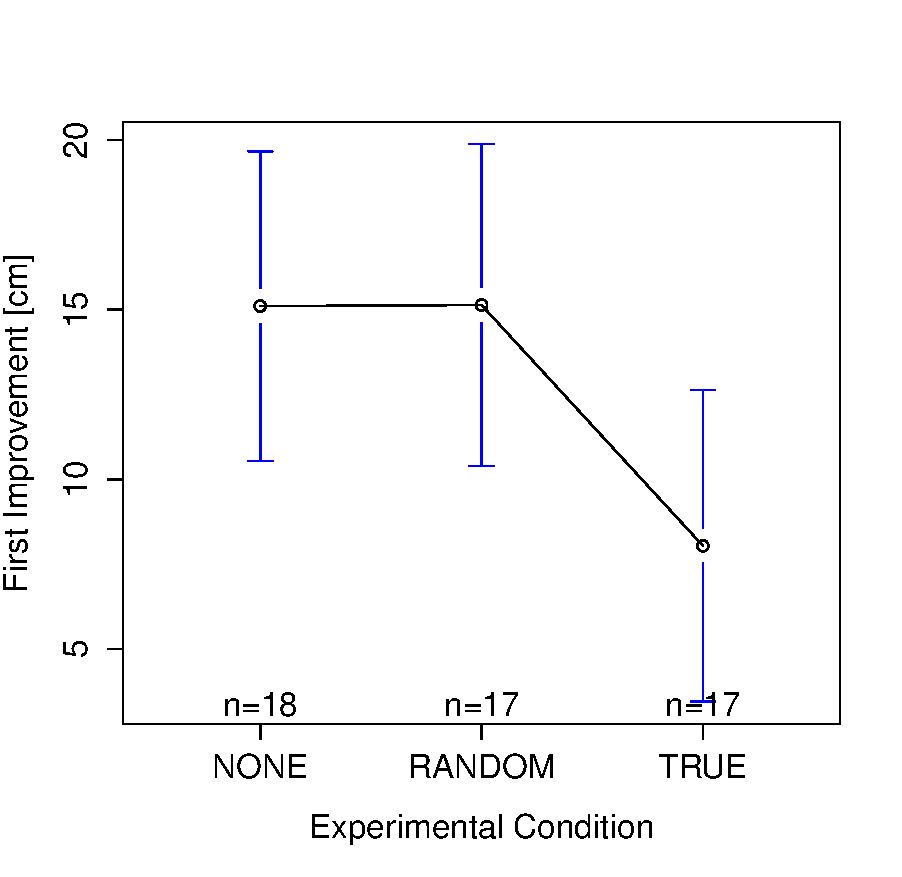
\includegraphics[width=0.8\linewidth]{meanPlotFirstImprove}
    \caption{First improvement vs.~experimental condition}
    \label{res2}
\end{figure}

\subsubsection{Average fixation duration on the reference side during interaction
phase vs.~condition}

The average fixation time on the reference side of the playground
(Figure~\ref{res3}) during the interaction phase is significantly more in {\sf NONE}
and {\sf RANDOM} condition than it is in the {\sf TRUE} condition ($F[2,49]=4.19$,
p = .02).

\begin{figure}[h!]
    \centering
    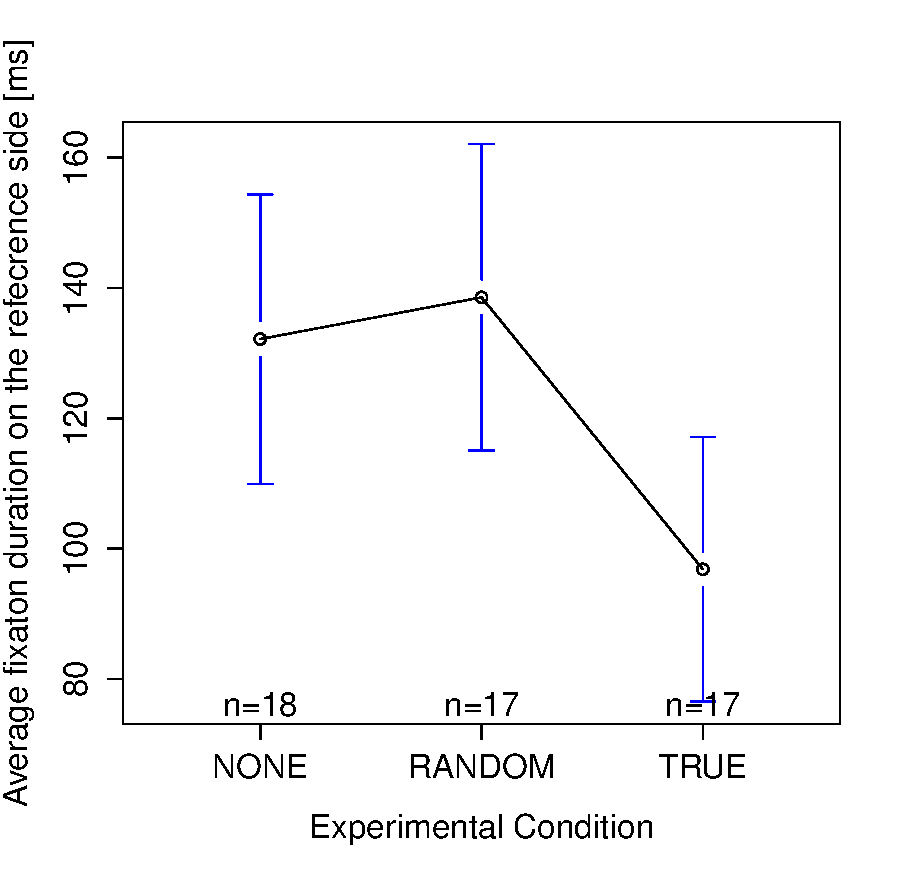
\includegraphics[width=0.8\linewidth]{meanPlotFixReference}
    \caption{Average fixation duration on the reference side during the
    interaction phase vs.~Condition}
    \label{res3}
\end{figure}

\subsubsection{First improvement vs number of fixations on reference side}

There is a significant negative correlation between the number of
fixations on the reference side (Figure~\ref{res4}) during the interaction phase
and the first Improvement ($t(50)=-2.13$, Pearson's correlation = -0.29, p=.03).

\begin{figure}[h!]
    \centering
    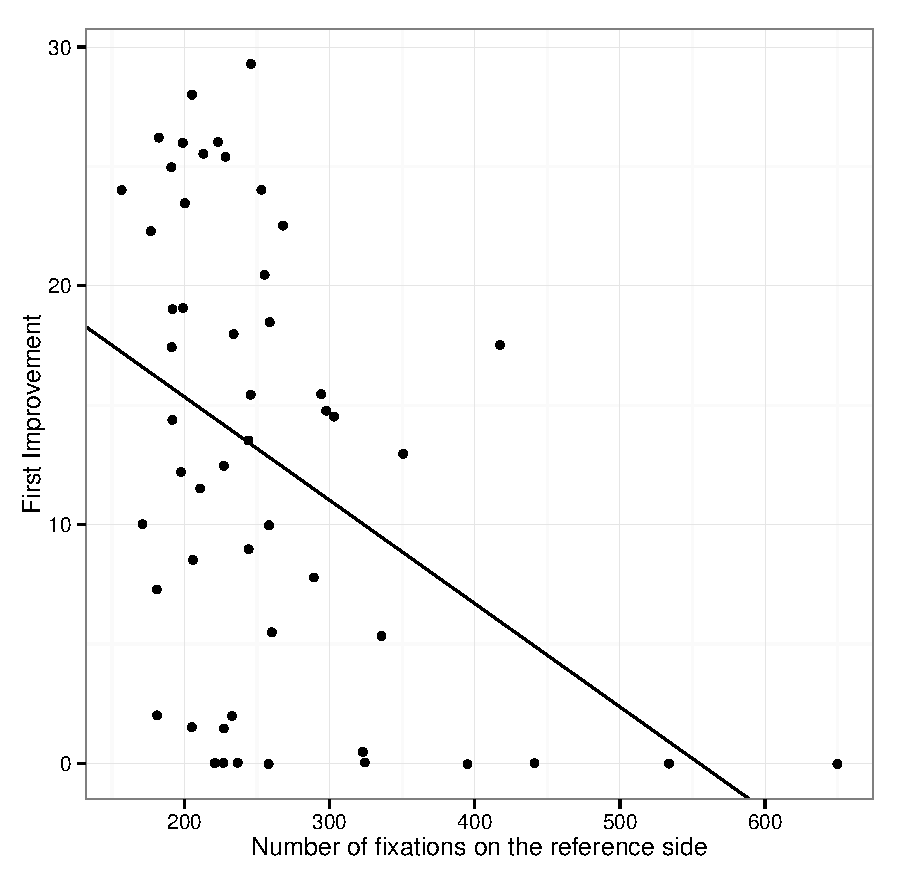
\includegraphics[width=0.8\linewidth]{corPlotFirstImprove}
    \caption{First improvement in centimeters ($y$-axis) vs.~number of fixations
    on reference side ($x$-axis) during the interaction phase.}
    \label{res4}
\end{figure}

%%%%%%%%%%%%%%%%%%%%%%%%%%%%%%%%%%%%%%%%%%%%%%%%%%%%%%%%%%%%%%%%%%%%%%%%%%%%%%%%%%%%
%%%%%%%%%%%%%%%%%%%%%%%%%%%%%%%%%%%%%%%%%%%%%%%%%%%%%%%%%%%%%%%%%%%%%%%%%%%%%%%%%%%%

\section{Interpreting the results}

We present an exemplar eye-tracking study in the context of human-robot
interaction within an educational setting. In this section we give an example of "how to interpret the eye-tracking results". The fact that participants have higher average fixation duration on the robot during the observation phase in the {\sf NONE} condition than the other two conditions (Figure 4) is not surprising as displaying visual information on the robot induces a saliency effect on the attention and the gaze is attracted towards the salient feature in the field of view. 

The fact that the participants in the {\sf RANDOM} or {\sf NONE} visualisation condition improved more than those with {\sf TRUE} condition is surprising (Figure 5). There are two plausible explanations. The first is that participants who see the robot in the {\sf TRUE} condition have a stronger belief that the robot always behaves the same. They see the LEDs of the robot turning on and therefore the robot still works. The ones with {\sf NONE} visualisation do not have an indication whether the robot works the same way as in the observation phase, and start experimenting earlier. The second explanation is that the participants in {\sf TRUE} condition just put the obstacles out of detection range, because they could see different display information and concluded therefore it may behave differently.







The fact that the participants in the {\sf RANDOM} or {\sf NONE} visualisation
condition improved more than those with {\sf TRUE} condition is surprising
(Figure 5). There are two plausible explanations. The first is that
participants who see the robot in the {\sf TRUE} condition have a stronger
belief that the robot always behaves the same. They see the LEDs of the
robot turning on and therefore the robot still works. The ones with {\sf NONE}
visualisation do not have an indication whether the robot works the same
way as in the observation phase, and start experimenting earlier. The
second is that the participants in {\sf TRUE} condition just put the obstacles
out of detection range, because they could see different display
information and concluded therefore it may behave differently.

The fact that participants have lower average fixation duration on the
reference side in the interaction phase in the {\sf TRUE} condition than the
other two conditions actually supports the explanation that participants
with {\sf TRUE} condition had a higher initial belief in their cognitive model
of how does the robot work (Figure 6). They did not need to look onto
the reference given in observation phase. This also verifies our working
hypothesis that a carefully designed mapping between the robot's
behaviour and its visual actuators can help in maximising the learning
effect during the interaction.

%Another plausible explanation for the participants in {\sf NONE} and {\sf RANDOM} condition
%being better performers than the {\sf TRUE} condition during the interaction phase
%comes from the transparency of the robot's behaviour. The robot's
%behaviour was not at all transparent in the former two conditions. This might
%have caused the participants to put more effort in understanding the behaviour.
%Therefore, they performed better.

\section{Conclusion}


We demonstrated that eye-tracking data can provide several process
variables to assess not only the task-based performance of the
participants but also to analyse HRI situations.

The advantages of mobile eye-tracking come with an additional cost. As
we mentioned earlier, the automatic localisation of the gaze pointer on
the visual stimulus is not a trivial task. To do this we have to use a
number of fiducial markers to the playground (Figure 2). We observed
that the fiducial markers cause a distraction to the participants. As a
future work, we are trying to find a suitable replacement to the
fiducial markers.



%%%%%%%%%%%%%%%%%%%%%%%%%%%%%%%%%%%%%%%%%%%%%%%%%%%%%%%%%%%%%%%%%%%%%%%%%%%%%%%%%%%%
%%%%%%%%%%%%%%%%%%%%%%%%%%%%%%%%%%%%%%%%%%%%%%%%%%%%%%%%%%%%%%%%%%%%%%%%%%%%%%%%%%%%



Our effort to use the confluent of eye tracking and human-robot
interaction provides insights to two aspects: first, as a way to
evaluate the human-robot interaction and second, as a way to evaluate
the interaction scenario.

%We addressed two research questions in the beginning of the present
%work. The results show that the way the sensor data is visualised has an
%impact on both the gaze patterns and the performance (Question 2).
%However, for the relation between the gaze patterns of the participants
%and their performance outcomes (Question 1) we cannot claim a direct
%relation. We found a negative correlation between the gaze-patterns and
%the first improvement during the interaction phase. We could not find a
%relation between the explanation of the participants and their
%gaze-patterns. Moreover, we did not find any anticipation patterns in
%the gaze data. The lack of evidence for the relation between
%participants' explanations and their gaze patterns prevents us to make
%any strong claims about the relation between the overall performance and
%the gaze patterns.
%
%The fact that we cannot find a relation between the gaze patterns and
%all the factors in the performance might have its roots in the way we
%designed the interaction phase experiment. As a working hypothesis we
%said that there should be clear and carefully designed mapping between
%the robots' behaviour and the sensor data visualization. Its environment
%also affects the behaviour of the robot and hence the environment also
%should be taken into consideration while designing the
%behavior-visualisation mapping. We introduced a novelty (the gray
%obstacle being more reflective) in the environment during the
%interaction phase of the experiment that forced the participants to
%revise their hypothesis and hence they failed to understand the robot's
%functionality. This also serves as a word of caution in future while
%designing such interactions. The observation phase serves as a training
%session for the participants, which can later be tested during the
%interaction phase. Any novel behaviour modality (in our case, the more
%reflective grey obstacle) can have a negative impact on the
%participants' understanding.

In a nutshell, the use of gaze data as an assessment of the human-robot
interaction in an educational setting provides future research
prospects. The data acquisition is a better trade-off between the
ecological validity of the experiment (as there cannot be an interaction
with the robot fMRI data acquisition) and the precision of the data
stream (wristbands for measuring the palpitation and the temperature).



%%%%%%%%%%%%%%%%%%%%%%%%%%%%%%%%%%%%%%%%%%%%%%%%%%%%%%%%%%%%%%%%%%%%%%%%%%%%%%%%%%%%
%%%%%%%%%%%%%%%%%%%%%%%%%%%%%%%%%%%%%%%%%%%%%%%%%%%%%%%%%%%%%%%%%%%%%%%%%%%%%%%%%%%%
% Removed for double-blind review
%\section*{Acknowledgments}
%
%This research was supported by...

%%%%%%%%%%%%%%%%%%%%%%%%%%%%%%%%%%%%%%%%%%%%%%%%%%%%%%%%%%%%%%%%%%%%%%%%%%%%%%%%%%%%
%%%%%%%%%%%%%%%%%%%%%%%%%%%%%%%%%%%%%%%%%%%%%%%%%%%%%%%%%%%%%%%%%%%%%%%%%%%%%%%%%%%%
\bibliographystyle{abbrv}
\bibliography{eyetracking}

\balancecolumns

\end{document}

